\begin{frame}{Citations}
    \begin{itemize}
        \item Regular (end) citation\cite{Fuller.2014}
        \item Footnote\footfullcite{Fuller.2019}
    \end{itemize}
\end{frame}

\begin{frame}{Reaction Classes and Examples}
    \begin{multicols}{2}
    \begin{itemize}
        \item Hydrogen abstractions
        \begin{itemize}
            \item \ce{RH} + \ce{NO2} $\rightleftharpoons$ \ce{R} + \ce{HONO}
            \item \ce{RH} + \ce{NO2} $\rightleftharpoons$ \ce{R} + \ce{HNO2}
            \item \ce{RH} + \ce{NO} $\rightleftharpoons$ \ce{R} + \ce{HNO}
        \end{itemize}
        \item Nitrite/Nitrate/Nitro-/Nitroso- Compounds
        \begin{itemize}
            \item \ce{RONO} $\rightleftharpoons$ \ce{RO} + \ce{NO}
            \item \ce{RONO2} $\rightleftharpoons$ \ce{RO} + \ce{NO2}
            \item \ce{RNO2} $\rightleftharpoons$ \ce{R} + \ce{NO2}
            \item \ce{RNO} $\rightleftharpoons$ \ce{R} + \ce{NO}
        \end{itemize}
        \item Isomerizations  
        \begin{itemize}
            \item \ce{RONO} $\rightleftharpoons$ \ce{RNO2}
        \end{itemize}
        \item \ce{HONO} elimination
        \begin{itemize}
            \item \ce{RONO} $\rightleftharpoons$ alkene + \ce{HONO}
        \end{itemize}
        \item \nox\ cycling
        \begin{itemize}
            \item \ce{RO2} + \ce{NO} $\rightleftharpoons$ \ce{RO} + \ce{NO2}
            \item \ce{R} + \ce{NO2} $\rightleftharpoons$ \ce{RO} + \ce{NO}
        \end{itemize}
    \end{itemize}
    
    \columnbreak
    
    \null \vfill
    \begin{figure}
        \centering
        \resizebox{\columnwidth}{!}{
            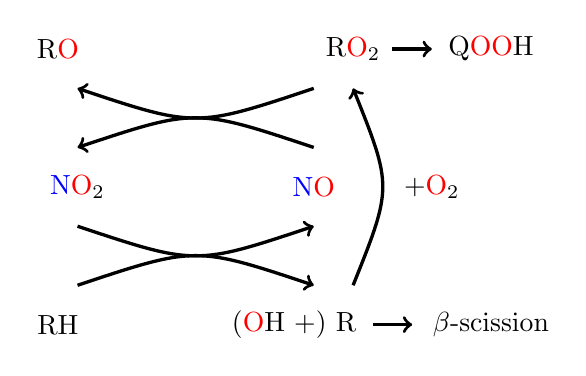
\begin{tikzpicture}
                %nox loop bounds
                \draw[->,very thick] (1,1) .. controls (2.5,0.5) .. (4,1);
                \draw[<-,very thick] (1,2) .. controls (2.5,2.5) .. (4,2);
                \draw (1,1.5) node {{\color{blue}N}{\color{red}O}$_2$};
                \draw (4,1.5) node {{\color{blue}N}{\color{red}O}};
                
                \draw[->,very thick] (1,0.25) .. controls (2.5,0.75) .. (4,0.25);
                \draw (0.75,-0.25) node {\ce{RH}};
                \draw (3.75,-0.25) node {({\color{red}O}H +) \ce{R} };
                
                \draw[<-,very thick] (1,2.75) .. controls (2.5,2.25) .. (4,2.75);
                \draw (0.75,3.25) node {R{\color{red}O}};
                \draw (4.5,3.25) node {R{\color{red}O}$_2$}; 
                
                \draw[->,very thick] (4.5,0.25) .. controls (5,1.5) .. (4.5,2.75); 
                \draw (5.5,1.5) node {+{\color{red}O}$_2$};
                
                \draw[->,very thick] (5,3.25)--(5.5,3.25); 
                \draw (6.25,3.25) node {Q{\color{red}O}{\color{red}O}H};
                
                \draw[->,very thick] (4.75,-0.25)--(5.25,-0.25); 
                \draw (6.25,-0.25) node {$\beta$-scission};
            \end{tikzpicture}
        }
        \caption{And when \ce{RH} is replaced with \ce{QOOH} or \ce{OOQOOH}?}
        \label{fig:NOx_cycle}
    \end{figure}
    \vfill \null
    
    \end{multicols}
\end{frame}

\begin{frame}{Progress on \nox-Cycling}
	\begin{figure}
		\centering
        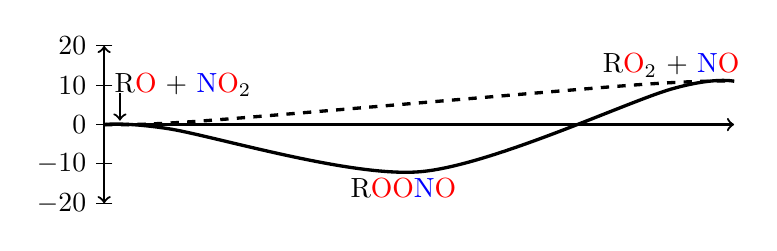
\begin{tikzpicture}[yscale = 0.5]
            %draw coordinate axis with labels
            %as above, not so many label, so they are manual here (e.g. make log)
            \draw[->,thick] (0,0) -- coordinate (x axis mid) (8,0);
            \draw[<->,thick] (0,2) -- coordinate (y axis mid)(0,-2);
            %\draw[gray, dashed](0,\ymax) grid (\Px,\ymin);
            \foreach \y/\ytext in {2/20, 1/10,0/0,-1/-10,-2/-20} \draw (3pt,\y cm) -- (-3pt,\y cm) node[anchor=east] {{$\ytext$}};
            
            %Text Labels
            %reactant side: placement will need to be adjusted for path lines
            \node [scale = 1.0,black] at (1.0, 1.0) {{R{\color{red}O} + {{\color{blue}N}{\color{red}O}$_2$}}};
            \node [scale = 1.0,black] at (7.2, 1.5){{R{\color{red}O}$_2$ + {{\color{blue}N}{\color{red}O}}}};      	
            \node [scale = 1.0,black] at (3.8, -1.60) {{R{\color{red}OO}{{\color{blue}N}{\color{red}O}}}};
            \draw[->,thick] (0.2,0.8) --(0.2,0.1);

            %links
            \draw[black, very thick] plot [smooth] coordinates {(0.0,0.0)(0.8,-0.1)(4.0, -1.2)(7.2,0.9)(8.0, 1.1)};
            \draw[black, very thick, dashed] plot [smooth] coordinates {(0.0,0.0)(1.3,0.1)(6.7,1.0)(8.0, 1.1)};
        \end{tikzpicture}
		\caption{Generalized potential energy surface for alkoxy radical (RO) + \ce{NO2} system. Energies in kcal/mol.
			Well-skipping occurs at virtually all combustion-relevant temperatures and pressures.}
		\label{fig:NOx-Cycle_PES}
	\end{figure}
\begin{tabular}{crrr}
	\toprule
	Reaction & \multicolumn{1}{c}{$A$} & \multicolumn{1}{c}{$n$} & \multicolumn{1}{c}{$E_a$}\\
	\midrule
	\ce{CH3O2} + \ce{NO} $\rightleftharpoons$ \ce{CH3O} + \ce{NO2} & 4.62E+15 & -0.38 & 97.8\\
	\ce{C2H5O2} + \ce{NO} $\rightleftharpoons$ \ce{C2H5O} + \ce{NO2} & 2.11E+14 & -0.12 & -470.6\\
	\ce{NC3H7O2} + \ce{NO} $\rightleftharpoons$ \ce{NC3H7O} + \ce{NO2} & 1.07E+14 & -0.25 & -1302.0\\
	\bottomrule
\end{tabular}	

Units: centimeters, kelvin, calories, moles
\end{frame}
